\section{审查、撤回与隔离项目改动}
\label{sec:ai-project-workflow}

当你开始让代理写入仓库，先学会用 Git 核对工作区、差异和分支，再用下面的练习比较桌面与终端的入口。运行构建和测试时，沿用卷一 CMake 章的流程。

\subsubsection{在桌面端审查差异与提交}
\label{sec:ai-desktop-review}

代理执行时，会在聊天中显示正在搜索、修改或运行什么。需要纠正方向就给出新的具体约束；需要停止则使用停止控件，随后检查已经产生的文件与进程。停止生成不等于撤销此前的改动。发送中的补充消息是立即引导当前工作还是排到下一轮，可在 Settings 的 Follow-up behavior 中设置，发送前留意界面提示。

在项目中通过 \textbf{New tab → Terminal} 打开集成终端。终端位于当前项目或 worktree，可用来独立运行构建命令、查看失败输出以及检查 \texttt{git status}。它不是另一个隔离副本；你在终端改文件，代理也会看到。把经常使用的构建、测试和启动命令配置为本地环境的 \textbf{Actions} 后，可以从顶栏快速执行；\textbf{Setup script} 则是在创建 worktree 时准备依赖的步骤，不应把启动开发服务器这种长期进程混进去。安装脚本、依赖和 Actions 本身也要检查，详见\href{https://learn.chatgpt.com/docs/environments/local-environment}{本地环境指南}。

代码改完以后，打开\textbf{差异面板（Diff / Review pane）}逐文件阅读。这里展示的是 Git 检出目录的状态，可能同时包含你自己、代理或其他工具的修改。按需切换 \textbf{Unstaged}、\textbf{Staged}、\textbf{Branch}、\textbf{Last turn} 等范围，别把“当前所有未提交改动”都算成代理刚刚写的。你可以对具体行留下评论，再在聊天中明确要求处理；也可以按块或按文件暂存、取消暂存、撤销修改。

\begin{figure}[!t]
    \centering
    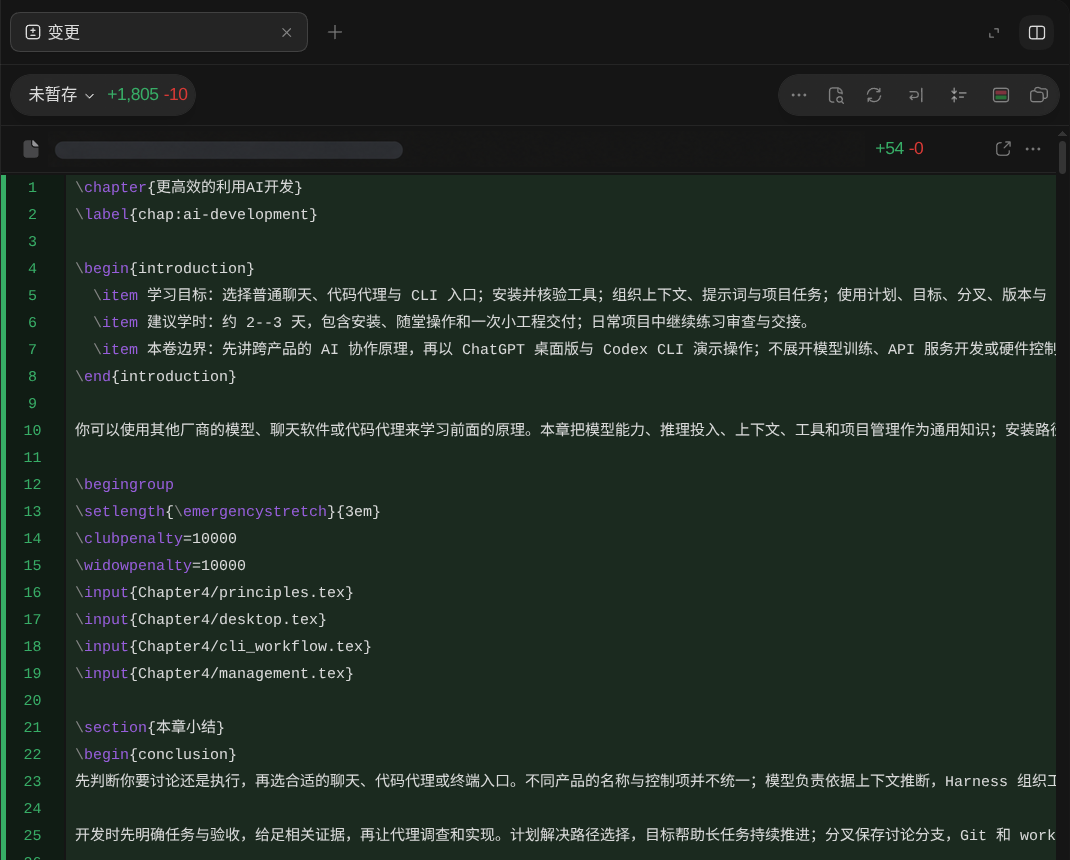
\includegraphics[width=0.92\textwidth]{images/ai/review-pane_revised.png}
    \caption{本机差异面板的真实局部截图。顶部“未暂存”表示查看范围，文件头与行号帮助定位，绿色部分是新增内容。文件路径以骨架占位脱敏，代码和计数保持原样；界面计数不是测试结果。}
    \label{fig:ai-review-pane}
\end{figure}
图~\ref{fig:ai-review-pane}~中整段为绿色，是因为这里正在查看新加入的教材文件。普通修改还可能出现删除行与修改块；先确认查看范围，再沿行号阅读，不能看到绿色就默认应该保留。

\texttt{/review} 会对选定范围进行代码审查并报告可疑问题。让它优先解释“什么输入触发、实际会怎样、预期应怎样、证据在哪”，再去核对代码与测试。审查没有发现问题，只表示这一轮没找到，不能替代构建、测试和实机验收。准备保留的改动确认后，再提交（Commit）；推送（Push）、创建 PR 和合并会影响远端，操作前要检查目标分支、内容与团队流程。\href{https://learn.chatgpt.com/docs/code-review}{审查指南}同时说明了本地审查与 PR 审查的区别。

\begin{note}
\textbf{Revert 会丢弃所选未提交改动。}先读差异，确认没有自己的工作被混在里面；需要保留的方案先提交到分支。对话分叉和文件回退的区别见本节后文，不能把聊天当作 Git 备份。
\end{note}

\Needspace{8\baselineskip}
\begin{example}[检查一个“看上去已经修好”的补丁]
让代理在练习副本中完成一个小改动后，先打开差异面板，确认只涉及任务所需文件；在关键行留下一条评论：“请解释空输入为什么走这条分支，并给出能覆盖它的命令。”发送后，核对解释与实际代码。

再在集成终端亲自执行项目 README 中的构建和相关测试命令。若失败，将完整命令、退出码与关键报错给代理，继续修复；通过后执行 \texttt{/review} 并选择未提交修改。最后检查差异、测试结果和已知限制，再暂存与提交。完成标志是一份你能解释且经过验证的补丁，而不是“AI 说它测过”。
\end{example}

\begin{exercise}\label{ex:ai-desktop-review}
在练习副本中检查一份补丁，找到一处关键逻辑并留下精确到行的反馈。记录一次实际验证的命令和结果，区分差异检查、AI 审查、运行测试分别能发现哪类问题。
\end{exercise}

\subsubsection{在 CLI 审查差异并复跑测试}

代码代理说“完成”以后，先用 \texttt{/diff} 看改动，再用 \texttt{/review} 请求审查。差异（Diff）展示文件内容的变化，审查（Review）尝试找行为问题、边界遗漏与测试缺口。两者都不能替你证明真实设备已经正常工作。普通终端的 \texttt{git diff} 也不会展示未跟踪文件的内容，因此还要看 \texttt{git status --short}，把新增源码一起读完。

审查提示最好给出检查对象与实际担心的故障。例如：“审查未提交改动，重点检查空输入、越界、单位和多线程退出；每个问题给出触发条件与文件位置，先不要修改。”如果你想审查分支相对主线的改动，就明确基线分支。不要让审查者只回答“写得很规范”。

\begin{example}[把一次修复变成可核对的交付]
让 Codex 完成练习工程中的一个小修改后，依次执行 \texttt{/diff}、\texttt{/review}。自己逐个读改动文件，运行 README 中的测试，再让它给出“修改内容、实际执行的检查、尚未验证的部分”。最后在普通终端用 \texttt{git status --short} 核对文件清单，只把你读懂且验证过的改动提交。提交消息应描述行为变化，例如“保留毫米换算的小数部分”，不要只有“AI 修改”。
\end{example}

当你已经把某类检查跑清楚，才考虑非交互执行。通用形式为 \texttt{codex exec [选项] "任务"}；它执行一次任务后退出，适合脚本或持续集成（Continuous Integration，CI），不适合把尚未定清的需求一股脑扔进去。下面只是只读检查示例，需在 Git 工程根目录执行，并使用没有占用的新输出路径：
\begin{tbash}
codex exec --sandbox read-only --json \
  --output-last-message /tmp/rm-ai-review.txt \
  "只读 README 与测试入口，列出检查命令和证据，不运行、不修改" \
  > /tmp/rm-ai-events.jsonl
\end{tbash}
\texttt{--json} 使标准输出包含逐行 JSON 事件，适合程序解析；\texttt{--output-last-message} 另外保存最终回复。Shell 重定向会覆盖同名文件，所以运行前先换成自己的新文件名。进程退出码只能说明这次执行的状态；最终回复中的“测试通过”仍要能追溯到实际测试输出。无人值守时遇到新的审批需求可能直接失败，应先在交互模式中验证权限与任务边界。

\begin{exercise}\label{ex:ai-cli-review}
对一次小修改完成差异审查，写出一条能触发错误的边界输入，以及一条证明修复的检查命令。解释为什么“CLI 正常退出”“审查未发现问题”“测试通过”不能互相替代。
\end{exercise}

\subsubsection{撤回文件改动前，先核对版本}
恢复或分叉聊天的入口见第~\ref{sec:ai-dialog-history}~节。做下面的练习前，先会看 Git 状态和差异，知道怎样保留自己的修改。

\begin{note}
\textbf{本节 Codex 的对话历史回退不会还原磁盘、Git 提交、外部服务或设备状态。}其历史回退接口只改会话历史。其他产品可能把回退与文件检查点绑定，操作前应读清确认框中的恢复范围，随后核对文件与进程；外部请求和设备动作仍需另查。若错误路线已经改了代码，先停下相关任务，检查 \texttt{git status} 与差异，再根据要保留的工作用 Git 处理；不要在带着他人改动的目录直接要求“全部恢复”。已提交的错误通常可以用 \texttt{git revert 提交号} 创建一个撤销提交，具体方法回看卷一第 1 章《Git 工具的使用》一节。
\end{note}

\begin{example}[用 Git 看清对话与文件分别发生了什么]
准备一份干净的 Git 练习副本，记录当前分支和提交。自己把计分器中 bonus 的初值改成 7 并保存。即使另开一个对话，改动仍在磁盘上。在练习仓库根目录核对：
\begin{tbash}
git status --short
git diff -- main.cpp
\end{tbash}
应看到 \texttt{main.cpp} 有一处未暂存改动。先决定该保留还是撤回，再按卷一 Git 一节处理，并重新核对差异。只处理这次练习的那一行；多人协作时，先分清哪些改动属于自己。
\end{example}

\begin{exercise}\label{ex:ai-workflow-history}
你在两个分叉中分别要求实现 A、B，结果它们修改了同一个源文件。解释原因，并写出继续实验前的处理步骤。另说明：如果已经把错误代码提交，对话回退后还缺哪一类操作？
\end{exercise}

\subsubsection{Worktree：让两条实现有各自的工作目录}

Git 工作树（Worktree）是同一仓库的另一份检出目录：各自有工作文件、暂存状态和检出位置，共享提交历史与对象数据库。它适合在稳定版旁边试一条新路线。Git 通常不允许同一个分支同时在两个 worktree 检出，所以要给实验使用独立分支。

本例桌面客户端的新对话可以在输入框下选择 \texttt{Worktree}，再选择起始分支；也可用 \texttt{/worktree}。Codex CLI 可从工程目录用 \texttt{codex --worktree} 创建托管 worktree。本例桌面客户端的托管工作树通常先处于游离 HEAD（Detached HEAD），准备长期保留成果时，用 \texttt{Create branch here} 建分支并提交。需要把对话及代码移回常用目录时，用 \texttt{Hand off} 到 \texttt{Local}，核对目标与差异再继续。不要另外在两个目录硬切同一个分支。

下面手动走一遍 Git worktree 的全过程，专门观察“分开修改，再审查合入”。命令不依赖 AI 账号，依赖前面 Git 一节已配置的提交身份。使用全新的练习目录；目录已存在就换名，并同步替换命令中的两个目录名。

\Needspace{14\baselineskip}
\begin{example}[用两个目录保留稳定版与候选版]
先在普通终端创建练习仓库：
\begin{tbash}
mkdir ~/rm-ai-worktree-lab
cd ~/rm-ai-worktree-lab
git init -b main
printf 'strategy=fifo\n' > policy.txt
git add policy.txt
git commit -m "记录队列策略基线"
git worktree add ../rm-ai-worktree-candidate -b codex/latest-frame
git worktree list
\end{tbash}
这里，\texttt{git worktree add} 后接新目录路径，用 \texttt{-b} 指定新分支。候选目录位于练习仓库旁边；列表应显示两个绝对目录，分别在 \texttt{main} 和 \texttt{codex/latest-frame}。

\Needspace{10\baselineskip}
然后只在候选目录修改、提交：
\begin{tbash}
cd ../rm-ai-worktree-candidate
printf 'strategy=latest\n' > policy.txt
git add policy.txt
git commit -m "试验最新帧策略"
cd ../rm-ai-worktree-lab
cat policy.txt
git diff main..codex/latest-frame -- policy.txt
\end{tbash}
此时主目录的内容仍是 \texttt{strategy=fifo}，差异里才会显示候选分支改成了 \texttt{latest}。换成真实项目时，两边必须各自在自己的目录构建和运行测试，构建目录也别混用。这里的文本只演示版本流转，不能证明某个队列实现正确。

\Needspace{8\baselineskip}
读完差异并确认要采用候选版后，在主目录执行：
\begin{tbash}
git merge --ff-only codex/latest-frame
cat policy.txt
git status --short
git worktree remove ../rm-ai-worktree-candidate
git branch -d codex/latest-frame
\end{tbash}
\texttt{--ff-only} 要求能直接快进才合入；真实工程出现分支分歧时它会拒绝，此时先审查并处理合并，不要照抄强制参数。文本应变成 \texttt{strategy=latest}，状态应干净。最后两条分别移除已无未提交改动的候选工作目录、删除已合入的实验分支；提交仍在主线历史中。
\end{example}

\begin{note}
移除 worktree 前，先停止使用该目录的代理、编辑器构建与后台程序，核对需要保留的改动已提交或另行保存。Git 拒绝移除脏目录时，先读原因，别立即加 \texttt{--force}。本例客户端托管的 worktree 可能随归档或清理被回收，长期成果应提交并推送到合适的仓库；其他工具的托管与回收规则需要另查。
\end{note}

Worktree 隔离的是检出文件，\textbf{不是虚拟机或安全沙箱}。两个目录仍可能共用相机、串口、GPU、数据库和网络端口；共享的外部服务写操作仍会冲突。Git 忽略的依赖、模型权重和本地配置也不一定自动出现在新目录。通过环境安装脚本准备依赖，敏感配置按需配置；不要为了让实验运行，把全部家目录、密钥或生产配置一并复制进去。

\Needspace{6\baselineskip}
\begin{conclusion}
对话分叉保留不同讨论路线；Git 分支保留代码历史；worktree 给不同检出各自的工作文件；沙箱限制工具能访问的资源。四者可以配合，不能互相替代。合并代码也不会自动合并两条聊天里的决定，采用的接口与验收结论还要写回项目记录。
\end{conclusion}

\Needspace{6\baselineskip}
\begin{exercise}\label{ex:ai-workflow-worktree}
按示例完成两个工作目录的创建、独立修改、差异审查、合入与清理。截取或保存合入前两个 \texttt{policy.txt} 的内容与 \texttt{git worktree list}；解释为什么两个 worktree 仍不能同时独占打开同一只相机。
\end{exercise}
